\documentclass[a4paper,10pt]{article}
\usepackage{a4wide}
\usepackage[english]{babel}
\usepackage{listings}
\usepackage{color}
\usepackage{mathtools}
\definecolor{Gray}{gray}{0.95}

% This is the list style for displaying C source code:
\lstdefinestyle{code}{
    language = C,					% The language of the code snippets
    basicstyle = \small\ttfamily,	% Font of the text
    numbers = left,					% Position of the line numbers
    numberstyle = \footnotesize,	% Style of line numbers
    frame = tb,				        % Style of surrounding frame
    framextopmargin=.75mm,         % Space margin top
    framexbottommargin=.75mm,      % Space margin bottom
    framexleftmargin=2mm,          % Space margin left
    framexrightmargin=2mm,         % Space margin right
    tabsize = 3,					% Size of tab character
    breaklines = true,             % Wrap lines of code that are too long
    columns = fullflexible,			
    showstringspaces = false,
    backgroundcolor = \color{Gray}
}

% This is the list style for displaying input/output. It is different from the style above, since you don't need C keywords to be highlighted in these listings. Line numbers are also emitted in this style.
\lstdefinestyle{stdio}{
    basicstyle = \small\ttfamily,	% Font of the text
    frame = tb,				        % Style of the surrounding frame
    framextopmargin=.75mm,         % Space margin top
    framexbottommargin=.75mm,      % Space margin bottom
    framexleftmargin=2mm,          % Space margin left
    framexrightmargin=2mm,         % Space margin right
    tabsize = 3,					% Size of tab character
    breaklines = true,             % Wrap lines of text that are too long
    columns = flexible,			
    showstringspaces = false,
    backgroundcolor = \color{Gray}
}

\title{Discs assignment}
\author{Y. Moustaghfir \& S. S. Hamed\\
        S2909758 \& S2562677}
%------------------------------------------------------------%
% This is where your document starts:

\begin{document}
\maketitle

\section{Problem description}
The program needs to calculate for a number of discs in a certain area the amount of discs that do not overlap each other. The input of the program would be first the amount of discs and after that the {\tt x} and {\tt y} and {\tt r}, which is the radius of the disc. The {\tt x} and {\tt y} value are coordinates for each disc. The precise definition of overlapping is that the discs are either on top of each other, which is of course obvious, or when the discs touch each other at the edges. 

\section{Problem analysis}
We start with looking at what we can do with our input. It seems that with the $x$ and $y$ coordinates we should be able to get the distance between two discs. First we compute the distance on the $x$ and $y$ axis between two discs. Let's call these $\Delta x$ and $\Delta y$. After we computed these we are able to use Pythagoras his method:
\begin{equation}
a^2 + b^2 =  c^2
\end{equation}
\begin{figure}[h]
\caption{Distance between discs that needs to be calculated}
\centering
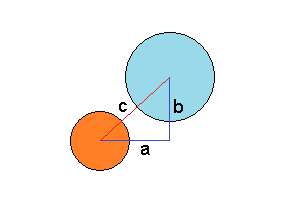
\includegraphics[width=0.5\textwidth]{img3.png}
\end{figure}
When using our coordinates it will be:
\begin{equation}
\Delta x^2 + \Delta y^2 = c^2
\end{equation}
with knowing $c^2$ we know the squared distance between the two centres of the discs. Now if we want to know if the discs overlap we need the other known input namely, the radius. We come out on the following equation:
\begin{equation}
if\:\:\:\ c^2 < (r_{1} + r_{2})^2\:\:\:discs\: overlap
\end{equation}
\begin{center}
\begin{minipage}{.6\textwidth}
\centering
and
\end{minipage}
\end{center} 
\begin{equation}
if\:\:\:\ c^2 \geq (r_{1} + r_{2})^2\:\:\:discs\: do\:not\:overlap
\end{equation}   
here $r_{1} \: and \: r_{2}$ are the two radius from the different discs.


\section{Design}
We start with our included {\tt safeMalloc} function to make sure that the memory is allocated correctly. After that we need to create a multidimensional array to store the values of each disc. 

In the {\tt makeDiscs} function, there is room for not just 3 int ({\tt x}, {\tt y} and {\tt z}), but also for a forth, which we will explain later. The next function calculates if there are discs that intersect. That is namely why the function is called {\tt intersect}. This function calculates the distance with the given array of coordinates and radius between to discs and the function is given two disc to calculate whether the two discs actually intersect or not. If this is the case, we store the value 1 in the variable {\tt count}. 

The next function is the {\tt countIntersect} function, which counts the different intersections between all the discs. The {\tt countIntersect} function has the input {\tt sz} and the array {\tt discs}. Given the size and the array, this function will loop over the array and after that, it will assign to each row(or each disc actually) a forth value if the two discs intersect. This forth value is to indicate whether the there has been an intersection between discs. If there is no forth value assigned to a certain disk, then there was no intersection between that disc and another. After that, we loop over each disc and increment the variable {\tt count} if there is a value found in the fourth index.

Then we end up in our main, where we ask the user for the input and store that in the array {\tt discs} and we store the size of the array in the variable {\tt sz}. After that we call our function to calculate the intersecting discs, and we print the number of discs and the number of non-overlapping discs. 


\section{Program code}
\begin{lstlisting}[style = code, title = discs.c]
/*
 * program: discs.c
 * 
 * Copyright 2015 Younes Moustaghfir, Sharif Hamed
 */ 

#include <stdio.h>
#include <stdlib.h>
#include <math.h>

void *safeMalloc(int size) {
  void *ptr = malloc(size);
  if (ptr == NULL) {
    printf("\nError: memory allocation failed....abort\n");
    exit(-1);
  }
  return ptr;
}

int **makeDiscs(int sz) {
  int row, **arr;
  arr = safeMalloc(sz*sizeof(int *));
  for (row=0; row<sz; row++) {
    arr[row] = safeMalloc(4*sizeof(int));
  }
  return arr;
}

int intersect(int disc1, int disc2, int **discs) {
	int sxD, syD, count = 0;
	int xD = discs[disc1][0] - discs[disc2][0];
	int yD = discs[disc1][1] - discs[disc2][1];
	sxD = xD * xD;
	syD = yD * yD;
	if(sxD + syD <= (discs[disc1][2]+discs[disc2][2])*(discs[disc1][2]+discs[disc2][2])) {
		count = 1;
	}
	return count;
}

int countIntersect(int sz, int **discs) {
	int count = 0;
	for(int i = 0; i < (sz-1); i++) {
		for(int j = i + 1; j < sz; j++) {
			if(intersect(i, j, discs)) {
				discs[i][3] = 1;
				discs[j][3] = 1;
			}
		}
	}
	for(int i = 0; i < sz; i++) {
		if(discs[i][3]) {
			count++;
		}
	}
	return count;
}



int main(int argc, char **argv)
{
	int count;
	int sz;
	int **discs;
	scanf("%d\n", &sz);
	discs = makeDiscs(sz);
	for(int i = 0; i < sz; i++) {
		scanf("%d %d %d\n", &discs[i][0], &discs[i][1], &discs[i][2]);
	}
	count = countIntersect(sz, discs);
	printf("number of discs: %d\n", sz);
	printf("number of non-overlapping discs: %d\n", sz-count);
	return 0;
}

\end{lstlisting}

\section{Test results}

\begin{itemize}

\item Input: First the size of the array, then coordinates and radius. ({\tt x}, {\tt y} and {\tt r})
\begin{lstlisting}[style = stdio]
10
  0   0   5
  1   7   1
  6   0   3
-12   9  10
  8   8   6
 15   3   4
 13   2   2
  7 -10   7
  3  15   2
 -9  -7   7
\end{lstlisting}

  Output:
\begin{lstlisting}[style = stdio]
number of discs: 10
number of non-overlapping discs: 3
\end{lstlisting}


\item Input:
\begin{lstlisting}[style = stdio]
5
  2   4   5
  3   7   1
-2   -3   3
-12   9  10
  9   5   6
\end{lstlisting}

  Output:
\begin{lstlisting}[style = stdio]
number of discs: 5
number of non-overlapping discs: 1
\end{lstlisting}


\item Input: 
\begin{lstlisting}[style = stdio]
3
 -5   3   4
  3  -7   1
 -2  -3   3
\end{lstlisting}

  Output:
\begin{lstlisting}[style = stdio]
number of discs: 
number of non-overlapping discs: 1
\end{lstlisting}

\end{itemize}

\section{Evaluation}
This assignment took us more time than expected. We understood the problem fast and also we knew how to solve it without using any  of angles(which was not given). The way to compute one comparison was not hard, but to make the loop work with a multidimensional-array took the longest.   
\end{document}
